\chapter{Experimental Results}

We conducted a series of experiments to evaluate both the performance of our proposed prediction error extraction algorithm and our new detection approach. In order to create a suitable dataset for our experiments, we gathered a set of at least 250 five second long video clips from a variety of camera models. Since the video processing pipeline is different between camera models, we aimed to include a diverse set of GOP structures. The list of camera models used to construct the dataset can be found in the first column of Table~\ref{datasetComp}. Data gathered from camera models with more than 275 videos was captured using multiple individual devices. The videos from the Google Pixel 1 contain footage captured on three devices, while the Kodak Ektra and Nokia 6.1 contain video from two devices. The dataset contains a total of 2728 unaltered videos.

To create our frame deleted videos, we then removed 15 frames from the beginning of each video in our unaltered video dataset. The reencoding was handled using the x264 library, and we matched the original GOP structure of each video for the frame deleted copy. We then filtered out all videos with less than 60 P-frames, as having fewer than 60 P-frames is not sufficient for making a reasonable classification of a video sequence. The resulting complete dataset can be found in Table~\ref{datasetComp}.

\begin{table}[htbp]
  \begin{adjustbox}{width=0.9\linewidth, center}
  \begin{tabu}{ l | l | c | c | c | c }
    \hline
    \rowfont{\bfseries} Camera Model & GOP Type & GOP N & GOP M & Genuine Videos & Frame Deleted Videos \\ \hline	
    ASUS ZenFone 3 Laser & Fixed & 30 & 1 & 257 & 257 \\
    Apple iPhone 8 plus & Variable & 30 & 2 & 248 & 245 \\
    Google Pixel 1 & Variable & 29 & 2 & 776 & 777 \\
    Google Pixel 2 & Variable & 29 & 2 & 212 & 212 \\
    Kodak Ektra & Fixed & 30 & 1 & 503 & 502 \\
    Nokia 6.1 & Fixed & 30 & 1 & 501 & 500 \\
    Samsung Galaxy S7 & Fixed & 30 & 1 & 231 & 231 \\ \hline
    \textbf{Total Count} &  &  &  & \textbf{2728} & \textbf{2724} \\ \hline
  \end{tabu}
  \end{adjustbox}
  \caption{Composition of Frame Deletion Dataset}
  \label{datasetComp}
\end{table}

Note that GOP N is the maximum distance between I-frames in a video, which is the GOP length. GOP M is the maximum distance between P-frames in a video, thus a video with an M value of 1 has no B-frames at all. Note that some deleted videos had just enough frames removed to put them below the 60 P-frame threshold. Thus, there is a slight imbalance between the total number of videos present in each class. The total number of videos with frame deletion is slightly less, at 2724 videos in total.

\section{Single Camera Model}

To gauge relative performance of our proposed detection methods, we first tested on a single camera model. We chose to use videos from the ASUS ZenFone 3 Laser. When testing for the effects of our proposed prediction error extraction method, we used the decision metric proposed by Stamm et al. \cite{stamm} for MPEG-2 video, as described in Equation~\ref{origdecision}. We varied the decision threshold used in each detector over a range of possible values. The probabilities of detection ($P_{D}$) and false alarm ($P_{FA}$) were measured for each value of the threshold. We then calculated the Receiver Operator Characteristic (ROC) curves for both prediction error extraction methodologies. The computed ROC curves can be found in Fig.~\ref{perrorExtractASUS}.
%
\begin{figure}[htbp]
\centerline{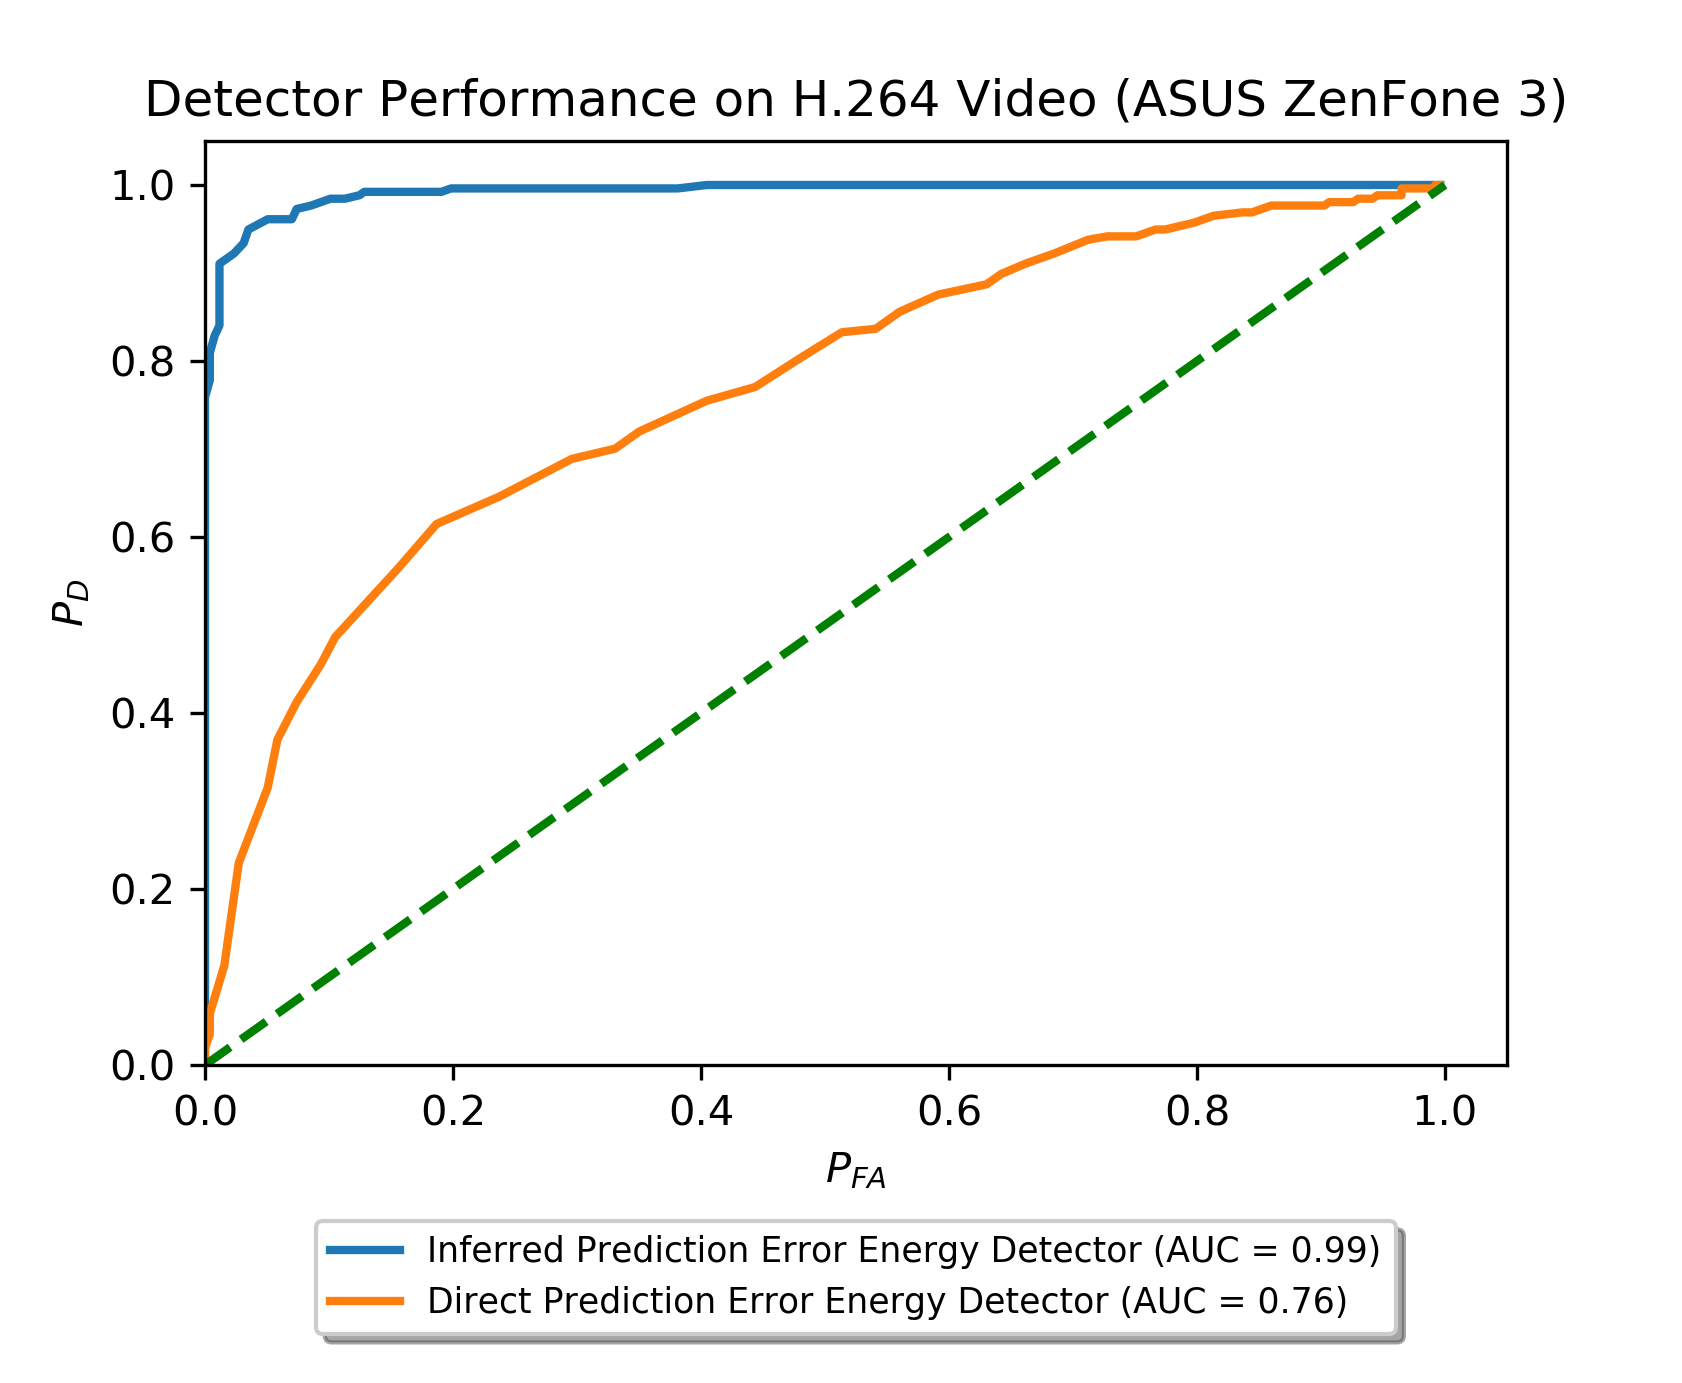
\includegraphics[width=0.7\linewidth]{ExperimentalResults/new_perror_extract_roc_asus.png}}
\caption{ROC Curves for Fingerprint Energy Detector Obtained by Using Different Prediction Error Extraction Methods}
\label{perrorExtractASUS}
\end{figure} 
%
As shown in Fig.~\ref{perrorExtractASUS}, extracting the prediction error sequence directly from the codec (direct prediction error) results in poor detector performance. The detector build from the direct prediction error sequence is only able to reach 60\% detection rates at 20\% false alarm rates. Compare to our proposed prediction error extraction methodology (inferred prediction error). For the ASUS ZenFone3, we achieve over 90\% detection rates at less than 10\% false alarm rates. These results indicate that indeed our new inferred prediction error extraction methodology is able to yield separation between the two classes of data where the original direct prediction error extraction methodology does not, particularly at low false alarm rates. There is a delta upwards of 70\% in the probability of detection for a given false alarm rate.
%
\begin{figure}[htbp]
\centerline{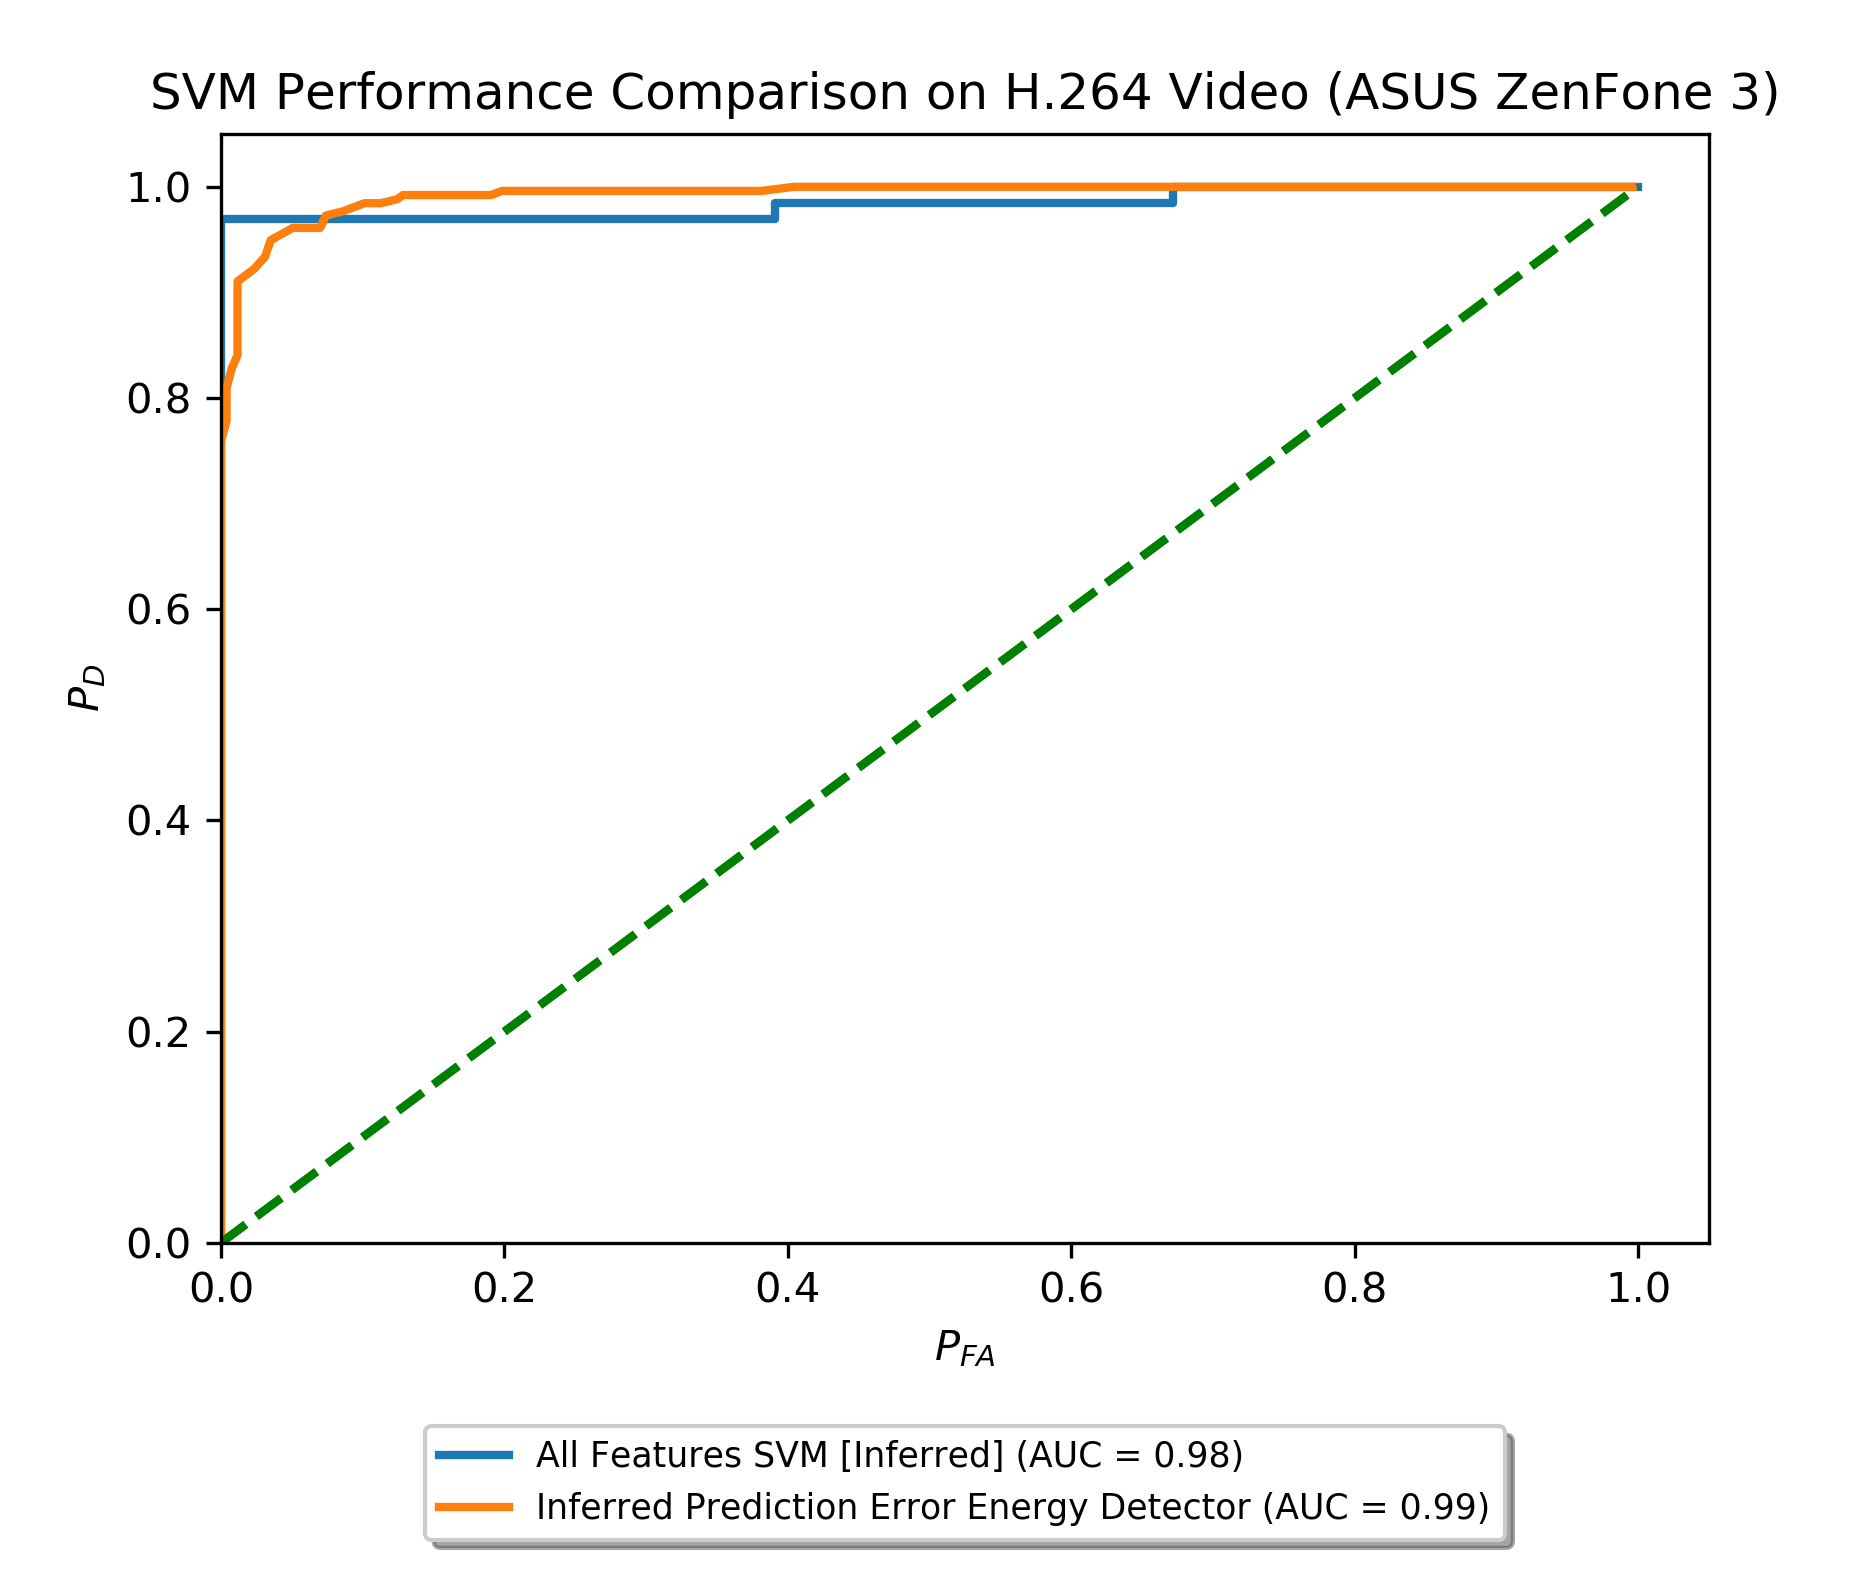
\includegraphics[width=0.7\linewidth]{ExperimentalResults/svm_perror_compare_roc.png}}
\caption{ROC Curves for Inferred Prediction Error Energy Detector and SVM on One Camera Model}
\label{svmrocASUS}
\end{figure}
%
Next, we examined the effects of using our proposed feature vector and an SVM on classification accuracy. We set the AR model orders for both the prediction error sequence and the fingerprint signal to 31. This is because of the periodic nature of the fingerprint on fixed GOP video. We want to predict when the signal will spike based on the previous GOP. We used the SVM with a radial basis function as the kernel and set the hyper-parameters of the SVM and the radial basis kernel to their defaults. To train the SVM, we partitioned our data into training and testing sets. The testing set was sized to be a quarter of the total dataset. Thus, there were 128 videos used for testing and 386 videos used for training. We set the SVM to use Platt scaling to return a probability instead of a class label \cite{plattscaling}. By doing so, we were able to vary the detection threshold and construct an ROC curve from the testing set for comparison with the fingerprint energy detector. The results can be seen in Fig.~\ref{svmrocASUS}.

As the detection rates for the fingerprint energy detector are already above 90\% for low false alarm rates, the relative magnitude of improvement when adding the SVM is less than when changing the prediction error extraction methodology. However, there is a significant improvement at false alarm rates under 10\%. The SVM detector is able to hold above 95\% accuracy at a 0\% false alarm rate. This suggests that some of the frame deleted videos do not have enough statistical differences from genuine videos to be classified as having frames removed from them. The videos in question may have low motion or content such that the fingerprint signal does not express itself in a detectable manner.

\section{Multiple Camera Models}

In order to obtain a better estimate of real world detector performance, we tested the effects of our proposed inferred prediction error extraction method using the entire dataset. We constructed ROC curves for detectors derived from both prediction error extraction methods. The resulting ROC curves can be seen in Fig.~\ref{perrorExtractFullDS}

It is obvious that the results obtained when testing solely on the ASUS ZenFone 3 were the best case scenarios for both prediction error extraction methods. In fact, using the direct prediction error extraction method from prior research does not yield much better detector performance than random chance. While not optimal, our proposed prediction error extractor provides a much cleaner separability of the data, even when confronted with a wide variety of videos. Without using the SVM, we are able to raise the probability of detection from 15\% to over 60\% at a 10\% false alarm rate.
%
\begin{figure}[htbp]
\centerline{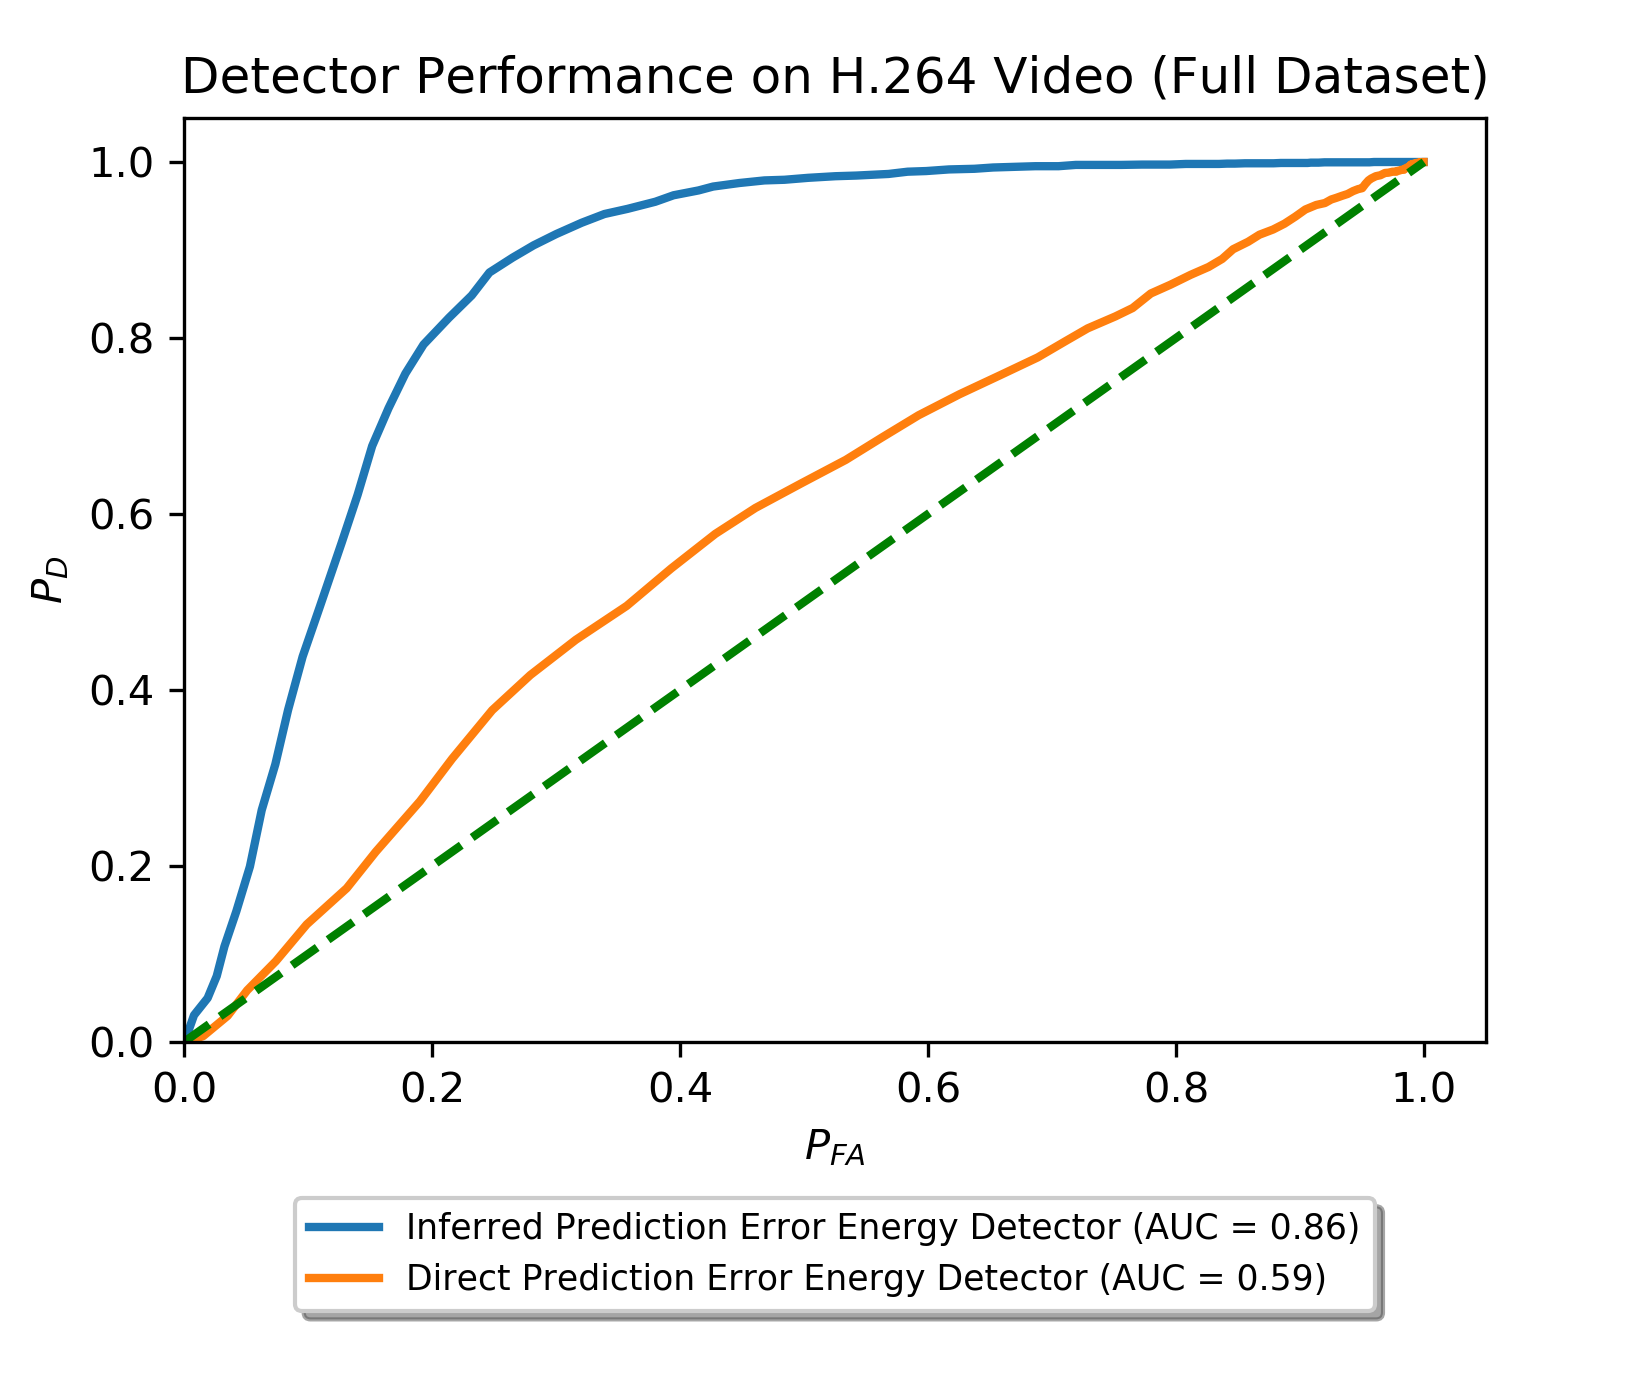
\includegraphics[width=0.7\linewidth]{ExperimentalResults/new_perror_extract_roc_full_ds.png}}
\caption{ROC Curves for Fingerprint Energy Detector Obtained by Using Different Prediction Error Extraction Methods on Multiple Camera Models}
\label{perrorExtractFullDS}
\end{figure} 

Before we tested the effects of our expanded feature vector and SVM on the entire dataset, we tuned the SVM to have optimal hyperparameters. We tuned both the penalty of the error term (C) and the size of gaussian used in the radial basis kernel (Gamma). We performed a grid search first in the log-scale to determine their optimal order of magnitude.
%
\begin{figure}[htbp]%
  \centering
  \subfloat[Log Scale Search for SVM Hyperparameters]{{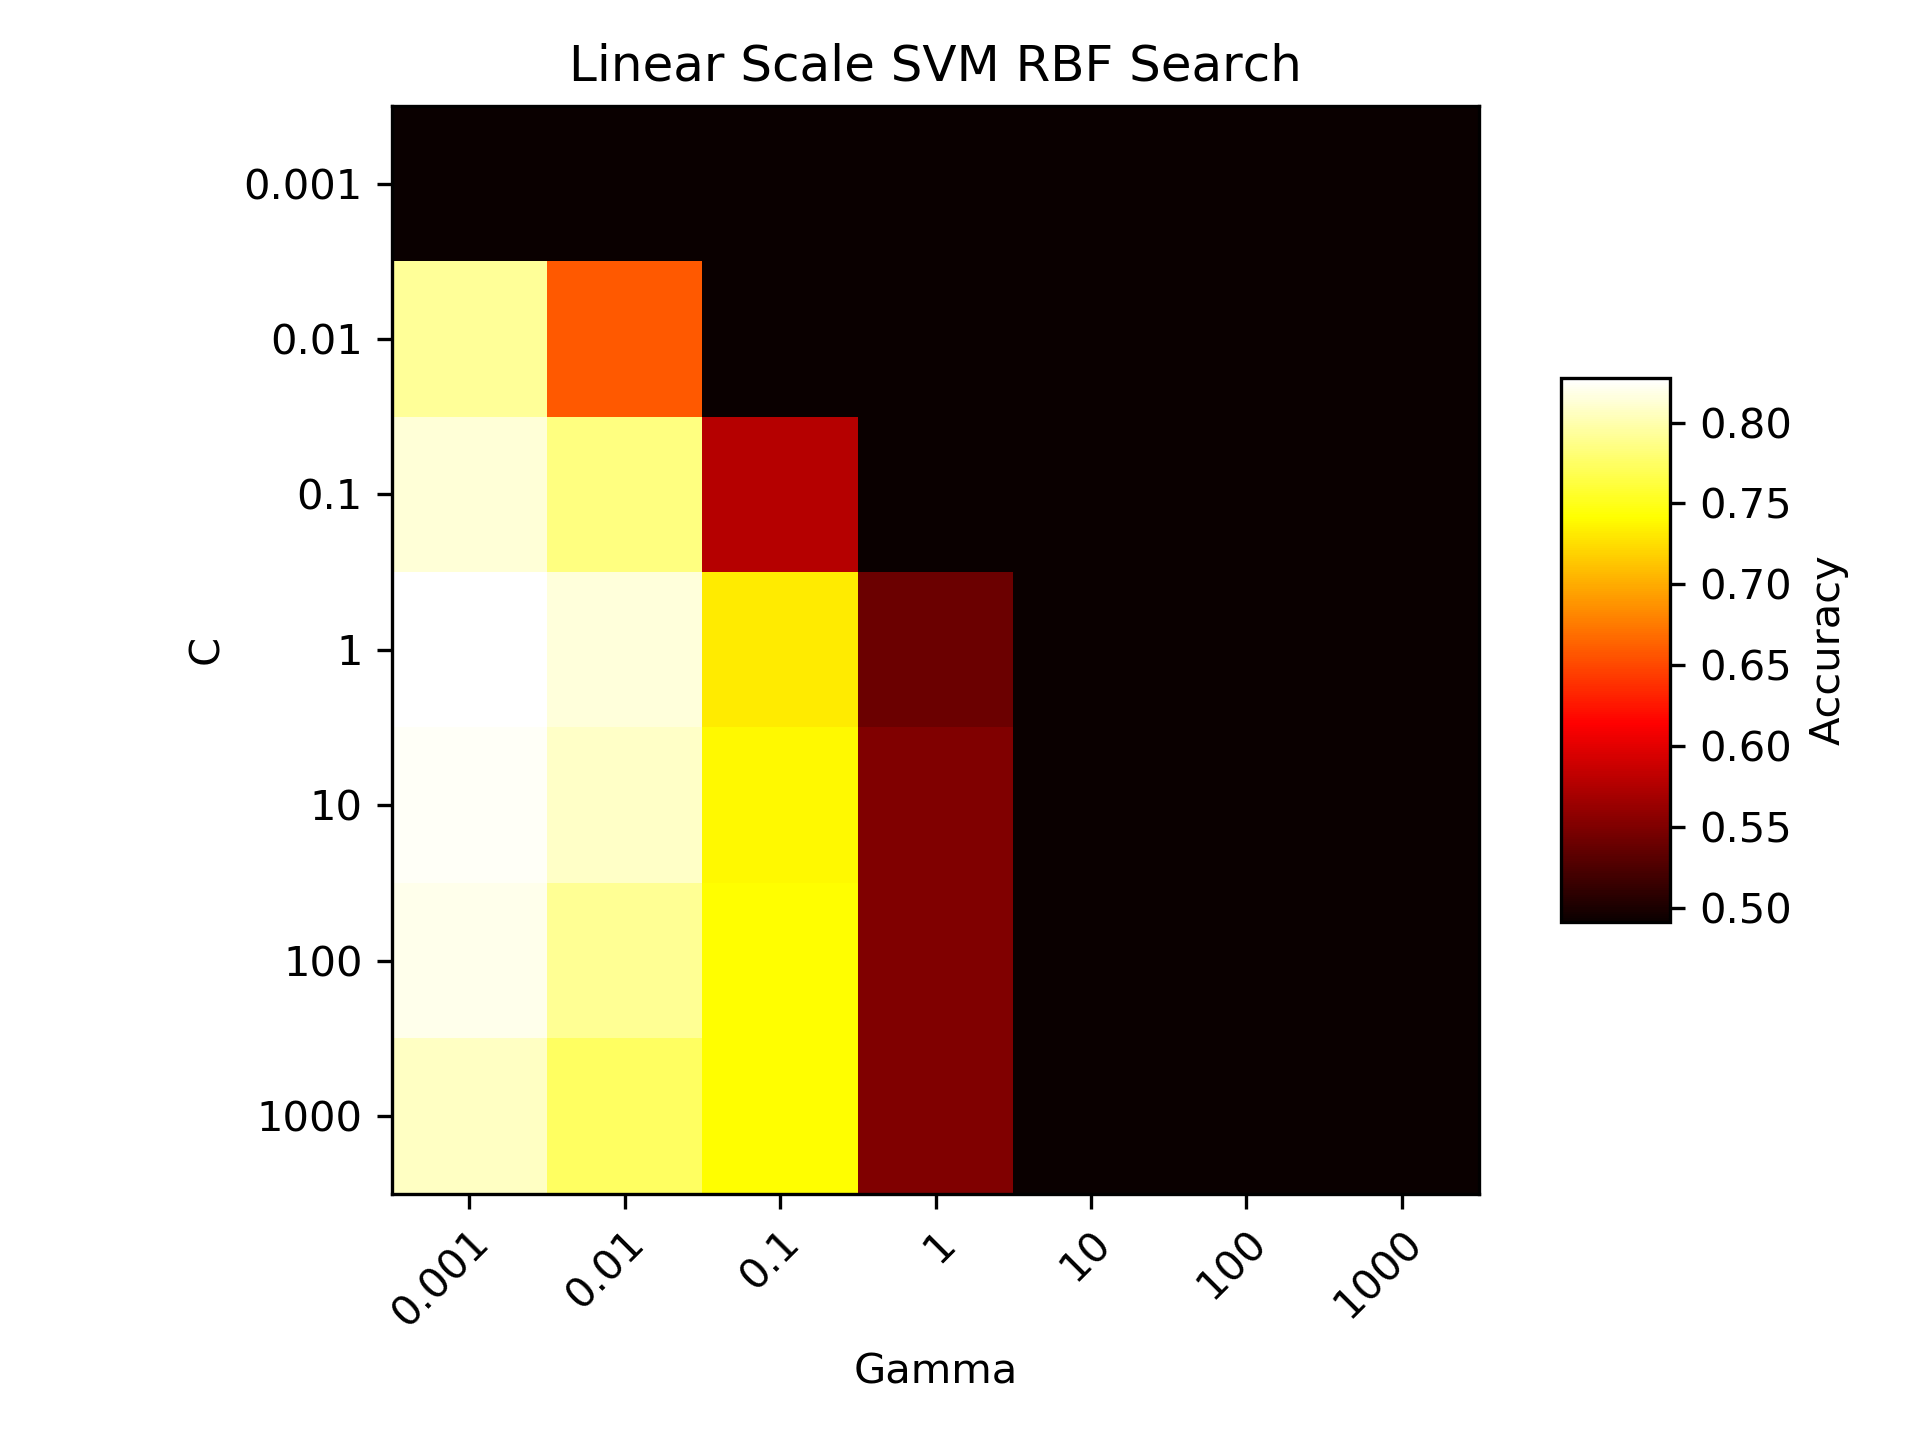
\includegraphics[height=5cm]{ExperimentalResults/log_scale_rbf_search.png}}}%
  \qquad
  \subfloat[Linear Scale Search for SVM Hyperparameters]{{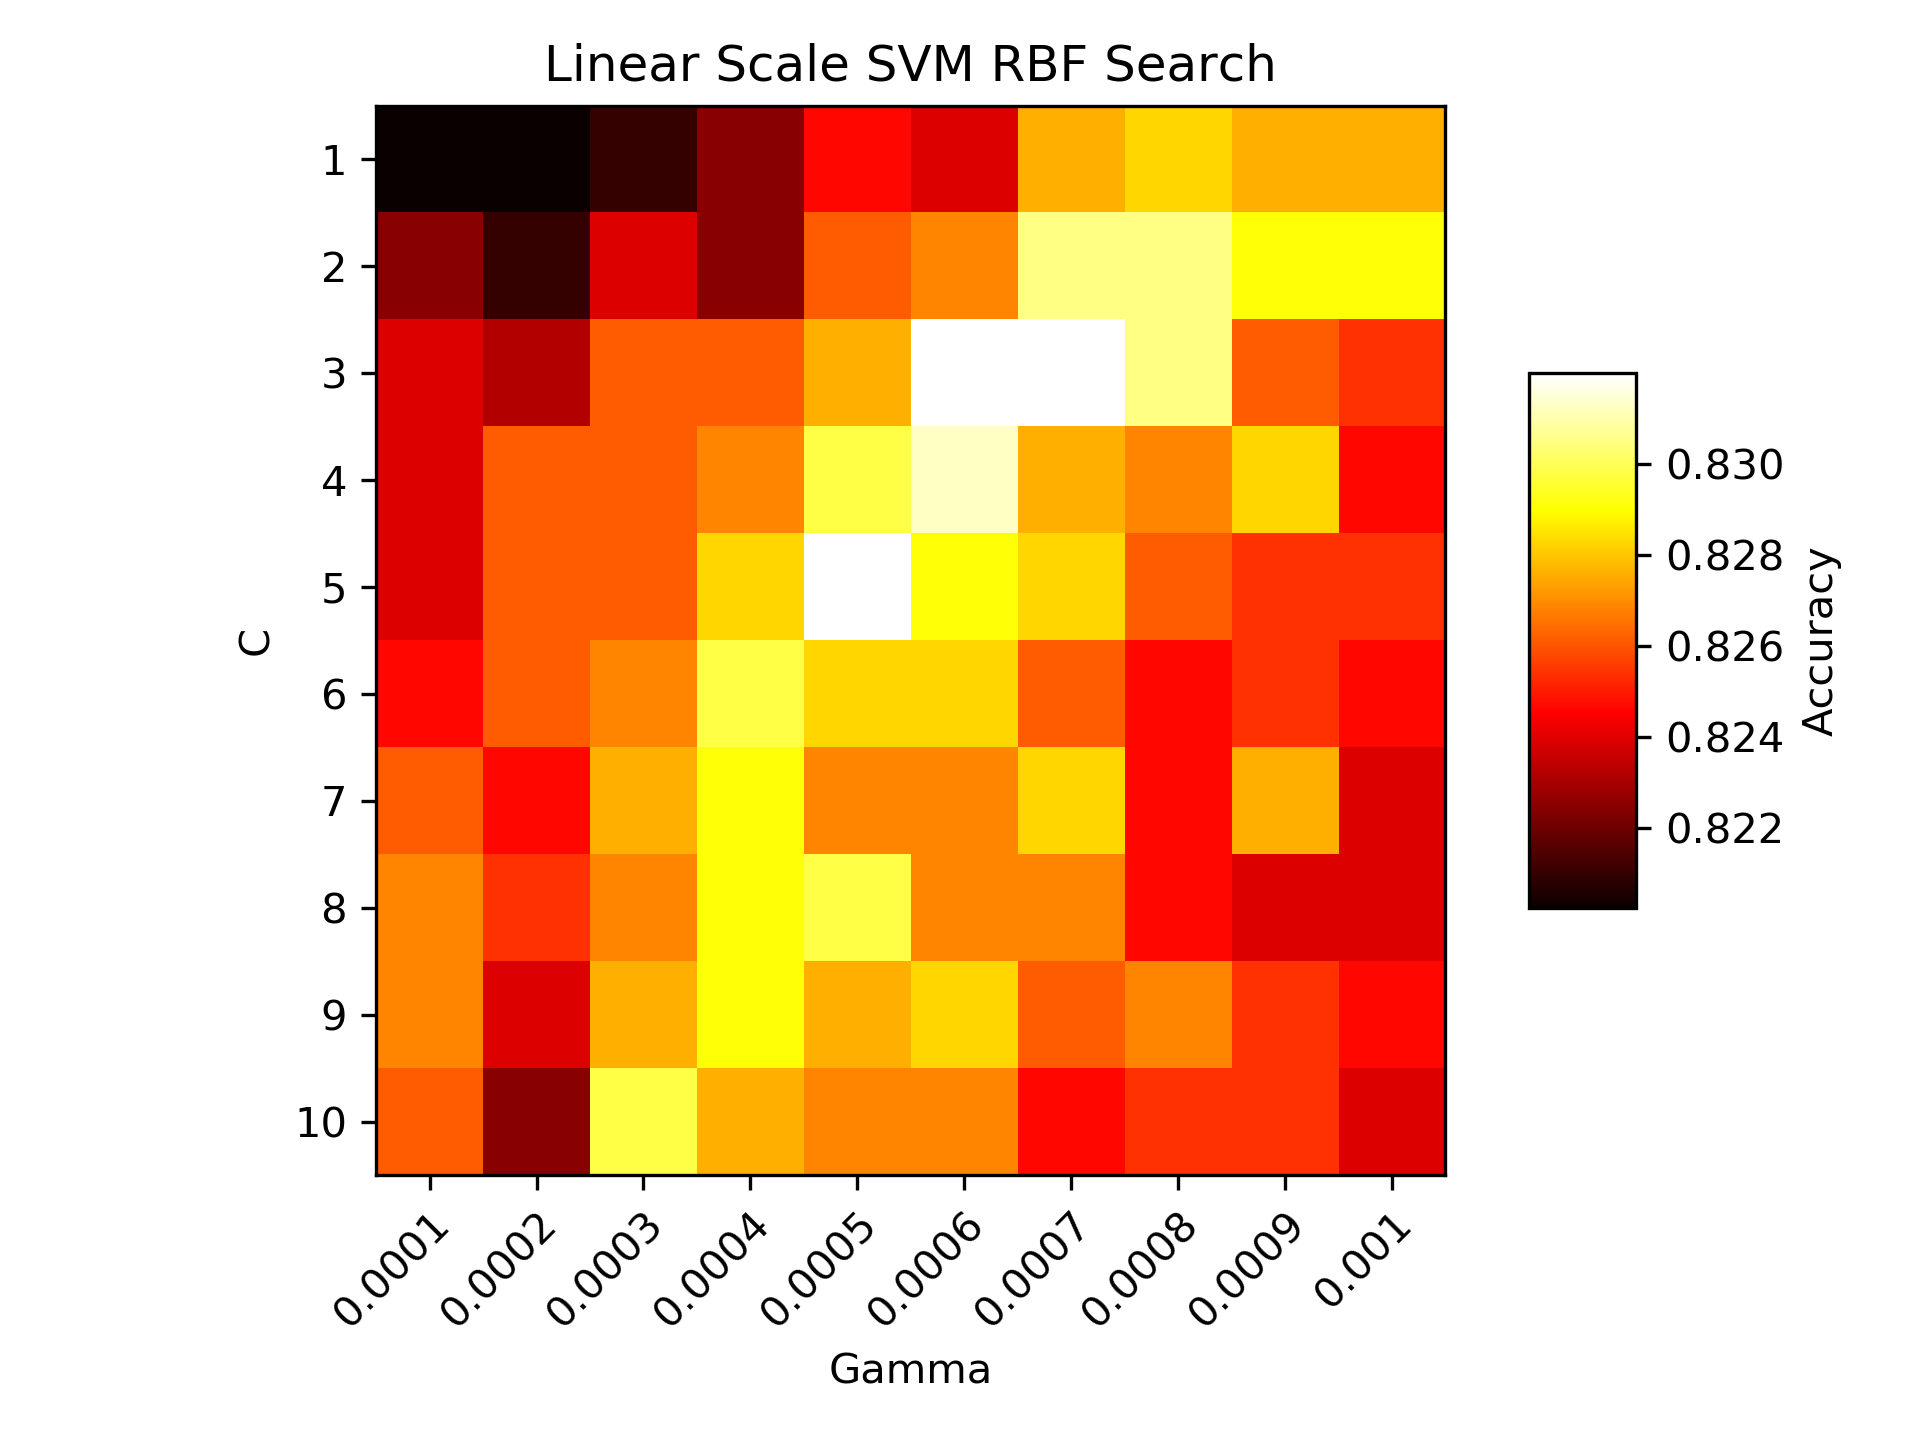
\includegraphics[height=5cm]{ExperimentalResults/lin_scale_rbf_search.png}}}%
\caption{Search for Optimal SVM Hyperparameters on (a) Log Scale and (b) Linear Scale}%
\label{svmparameters}%
\end{figure}

After determining the optimal order of magnitude for both of the hyperparameters, we performed a second grid search, but on a linear scale to find the set of optimal parameters. Fig~\ref{svmparameters} shows the results of both the log and linear scale grid searches. We chose to use $C = 5$ and $Gamma = 0.0005$ for our SVM. As we did previously, we split our entire dataset into training and testing sets to evaluate the SVM, where the testing set consisted of a quarter of the data. The dataset was shuffled prior to splitting so that a sampling of all camera models would be included in the testing set. Fig.~\ref{fullDSSVM} shows the ROC curves for the fingerprint energy detectors for both the direct and inferred prediction error extraction methods as well as SVMs.
%
\begin{figure}[htbp]
\centerline{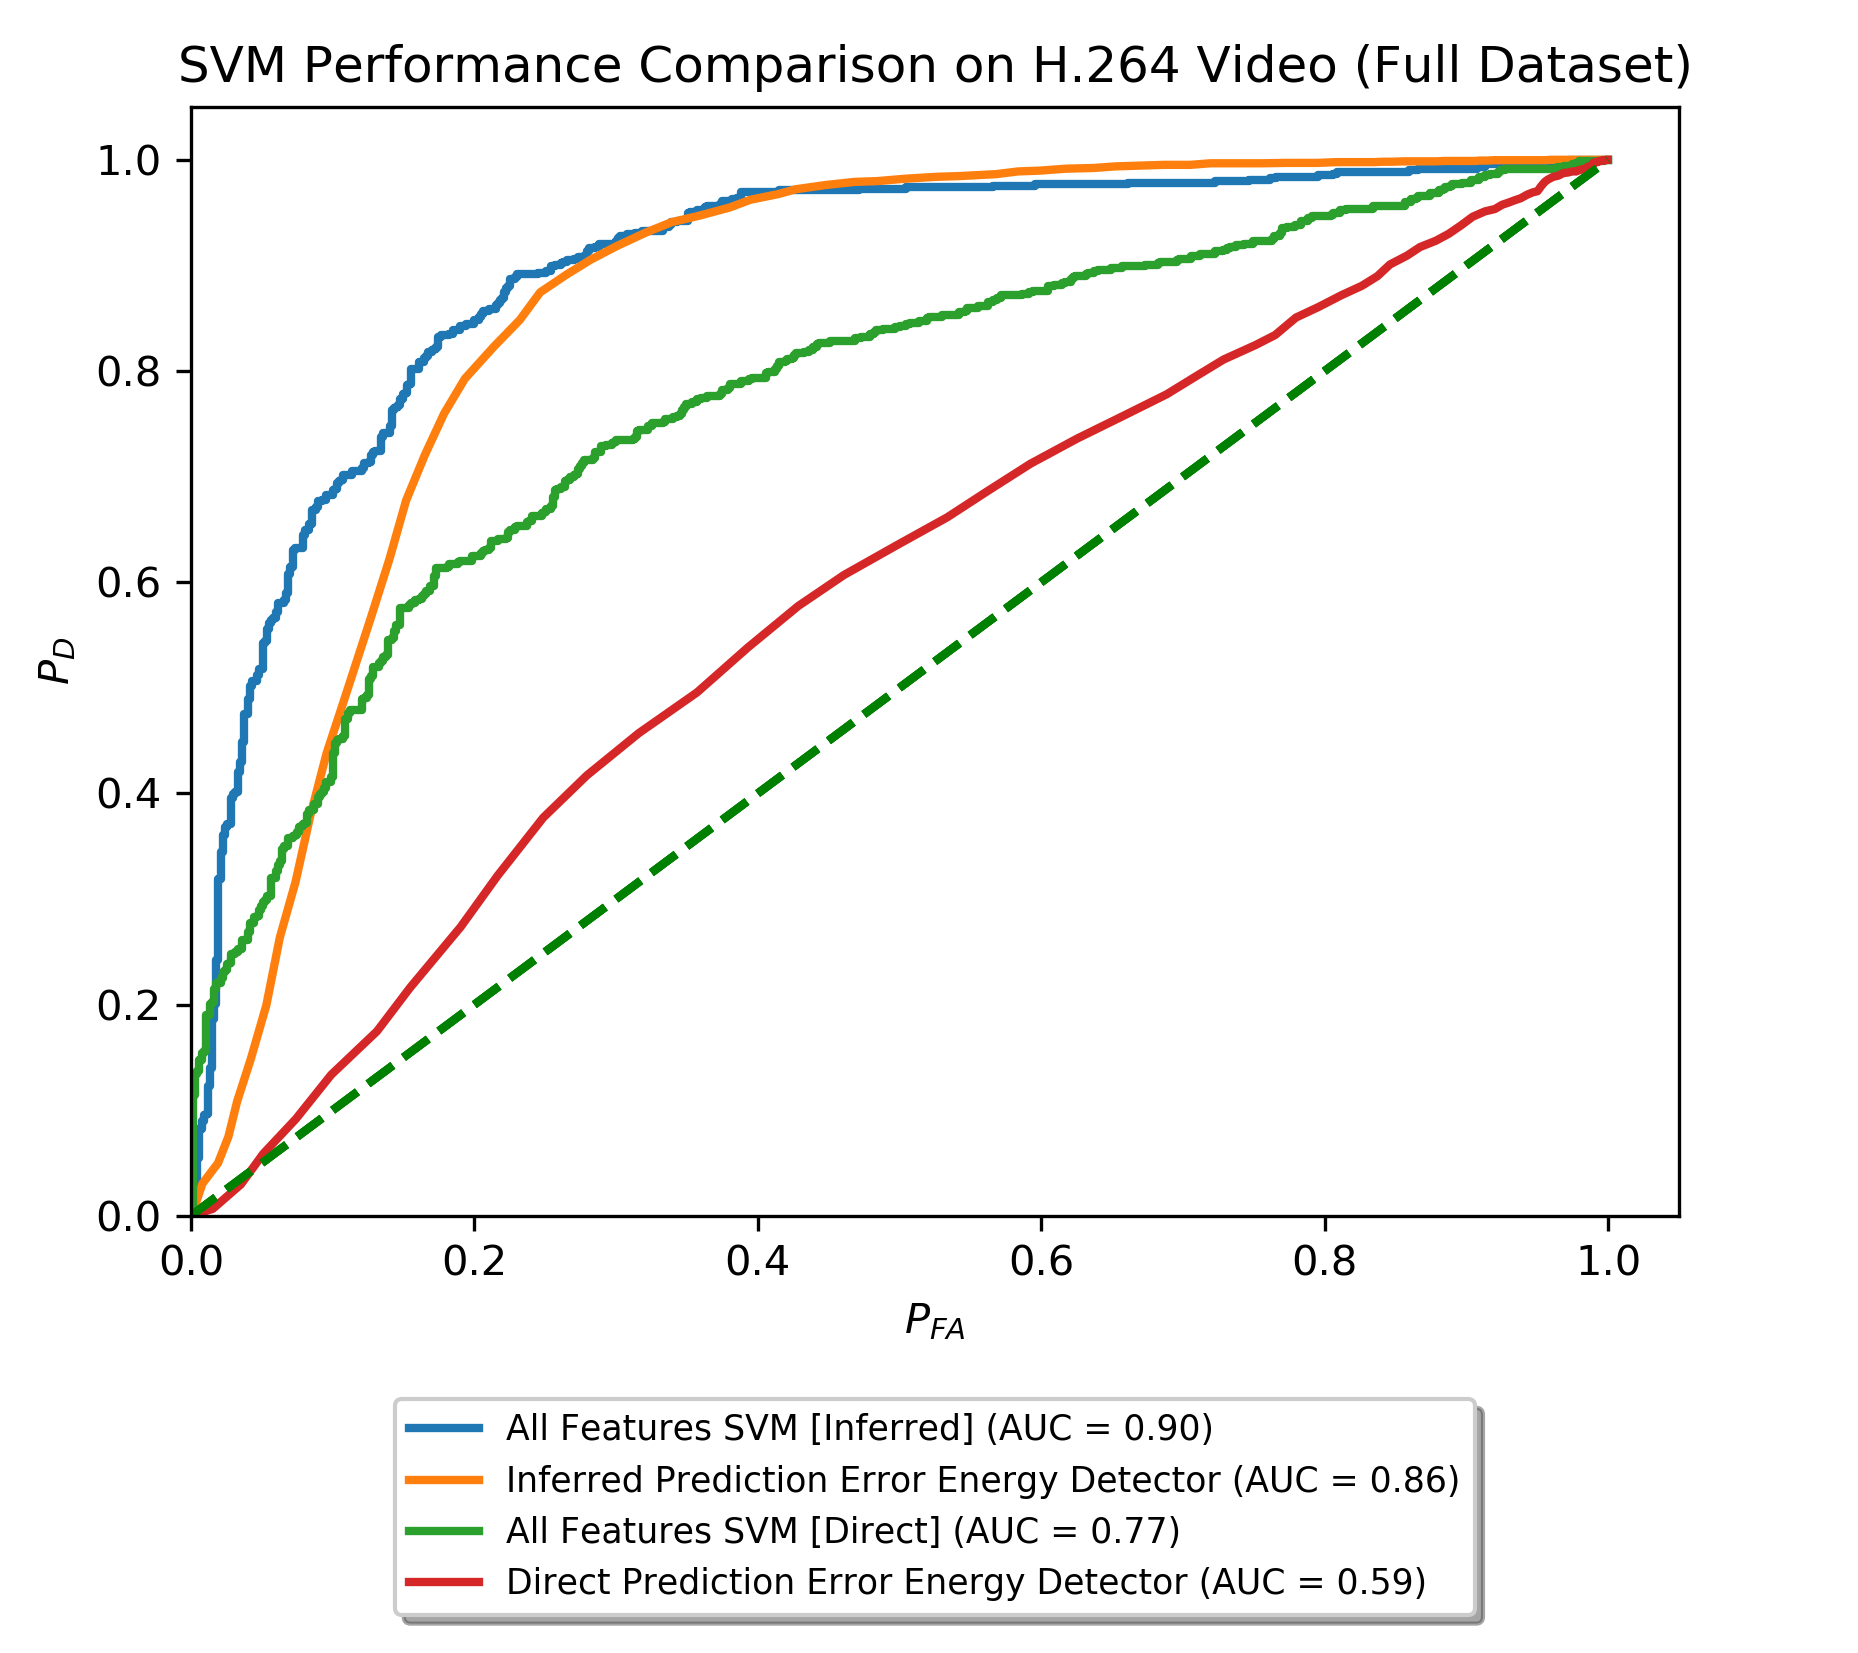
\includegraphics[width=0.7\linewidth]{ExperimentalResults/full_ds_compare_roc.png}}
\caption{ROC Curves for Various Detection Methods on Data from Multiple Camera Models}
\label{fullDSSVM}
\end{figure}

Using our proposed feature vector and SVM with the direct prediction error extraction method allows for some discrimination between the classes. However, the overall detector performance is still less than that of the fingerprint energy detector using our proposed inferred prediction error extraction methodology. Using our proposed feature vector and SVM with our proposed inferred prediction error extraction methodology yields the best detector performance in this scenario, particularly at low false alarm rates. At a 10\% false alarm rate, our combined detector yields an almost 80\% probability of detection.

\section{Additional Work}

As we have shown, our proposed detector is able to distinguish between genuine videos and videos with frame deletion with a reasonable level of accuracy. Indeed, it is also more effective than previously formulated motion vector based detectors, particularly those formulated for use on MPEG-2. However, this is only in a fairly limited scenario. Many videos, especially those shared on social media, are often recompressed, even without having frames removed from them. These videos often exhibit similar traces to videos with frame deletion. Thus, we tested our proposed detector on an additional classification problem. Given a feature vector $\bm{x}$ was originally found to have frame deletion, it belongs to one of two classes:%
%
\begin{equation}
\begin{aligned}
  C_{0} &: \bm{x} \text{ resulted from an altered video which has had frames removed from it.} \\
  C_{1} &: \bm{x} \text{ resulted from a video that has been recompressed without having frames removed.}
\end{aligned}
\end{equation}
%
\begin{figure}[htbp]
\centerline{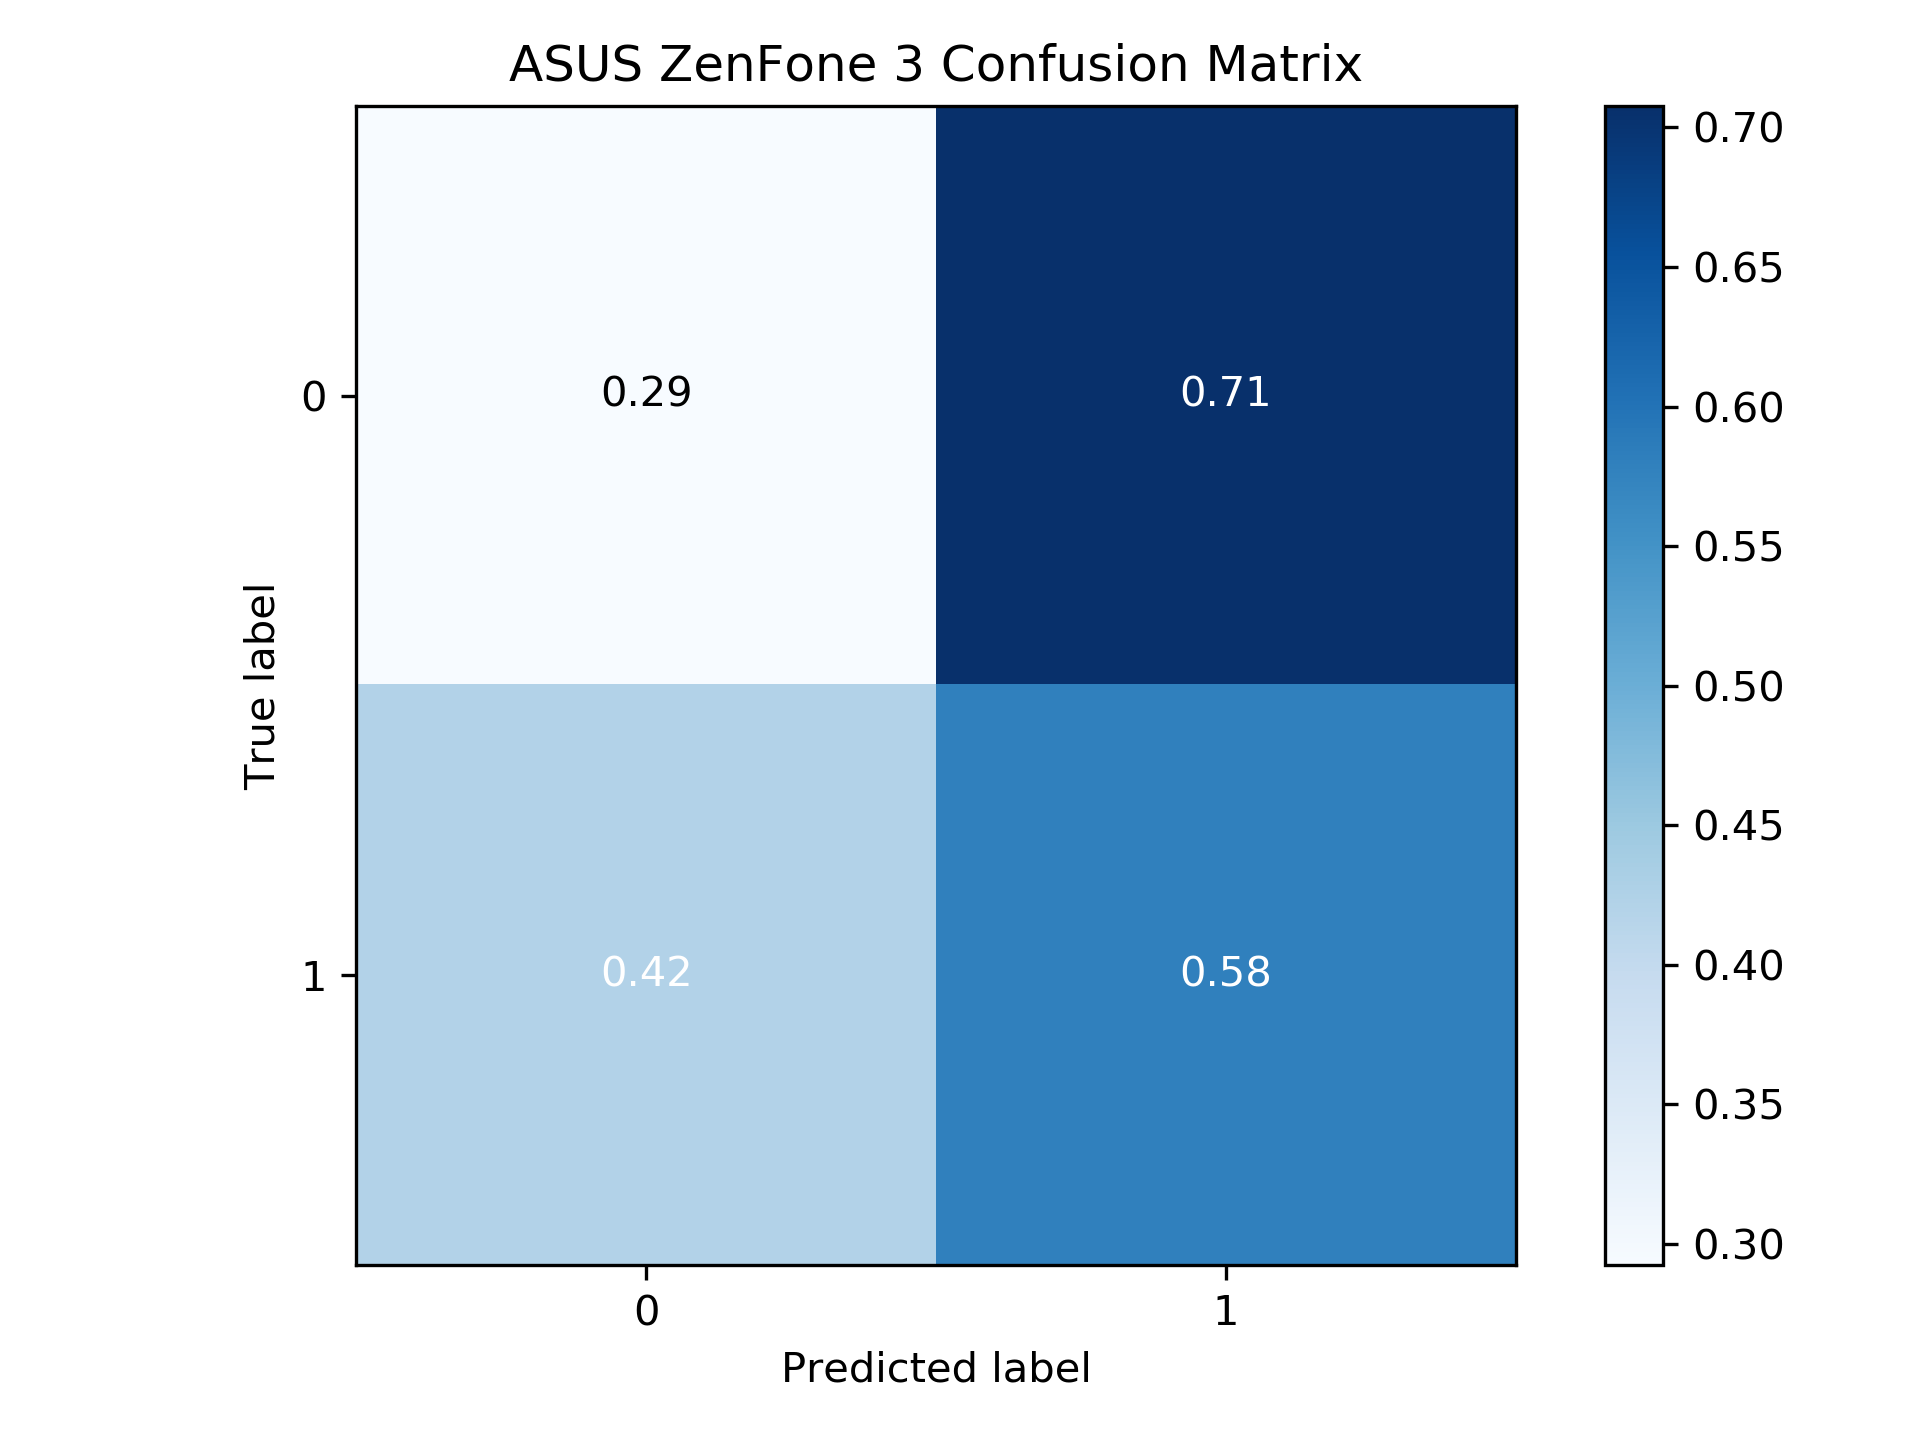
\includegraphics[width=0.67\linewidth]{ExperimentalResults/normal_cm.png}}
\caption{Confusion Matrix for Recompression Classification}
\label{normalcm}
\end{figure}

To test this, we created a third set of videos for the ASUS ZenFone 3, where each unaltered video in the dataset was recompressed. Thus we had a dataset of 257 videos for each class. We trained our SVM using the same training and testing data ratio as above, and used the same SVM parameters. We tabulated our results into the confusion matrix in Fig.~\ref{normalcm}.

From this confusion matrix, it becomes clear that more work is needed on our proposed detector. We are able to very easily distinguish whether videos have been recompressed or not, but it is a much more difficult problem to pinpoint the differences between videos that have had frames removed and videos that have only been recompressed. Additional work is needed to make an explicit detector for this scenario.

It is possible to tune our proposed detector slightly to increase the overall accuracy of the system. If we scale our data to have zero mean and unit variance on a feature by feature basis, we can trade some accuracy in the genuine class for better distinction between videos with frame deletion and recompressed videos. Fig.~\ref{scaledcm} shows that we can now separate videos with frame deletion and recompressed videos. Using additional features or a more complex system that can learn spacial relationships like a Convolutional Neural Network (CNN) should be able to fully separate these two classes.
%
\begin{figure}[htbp]
\centerline{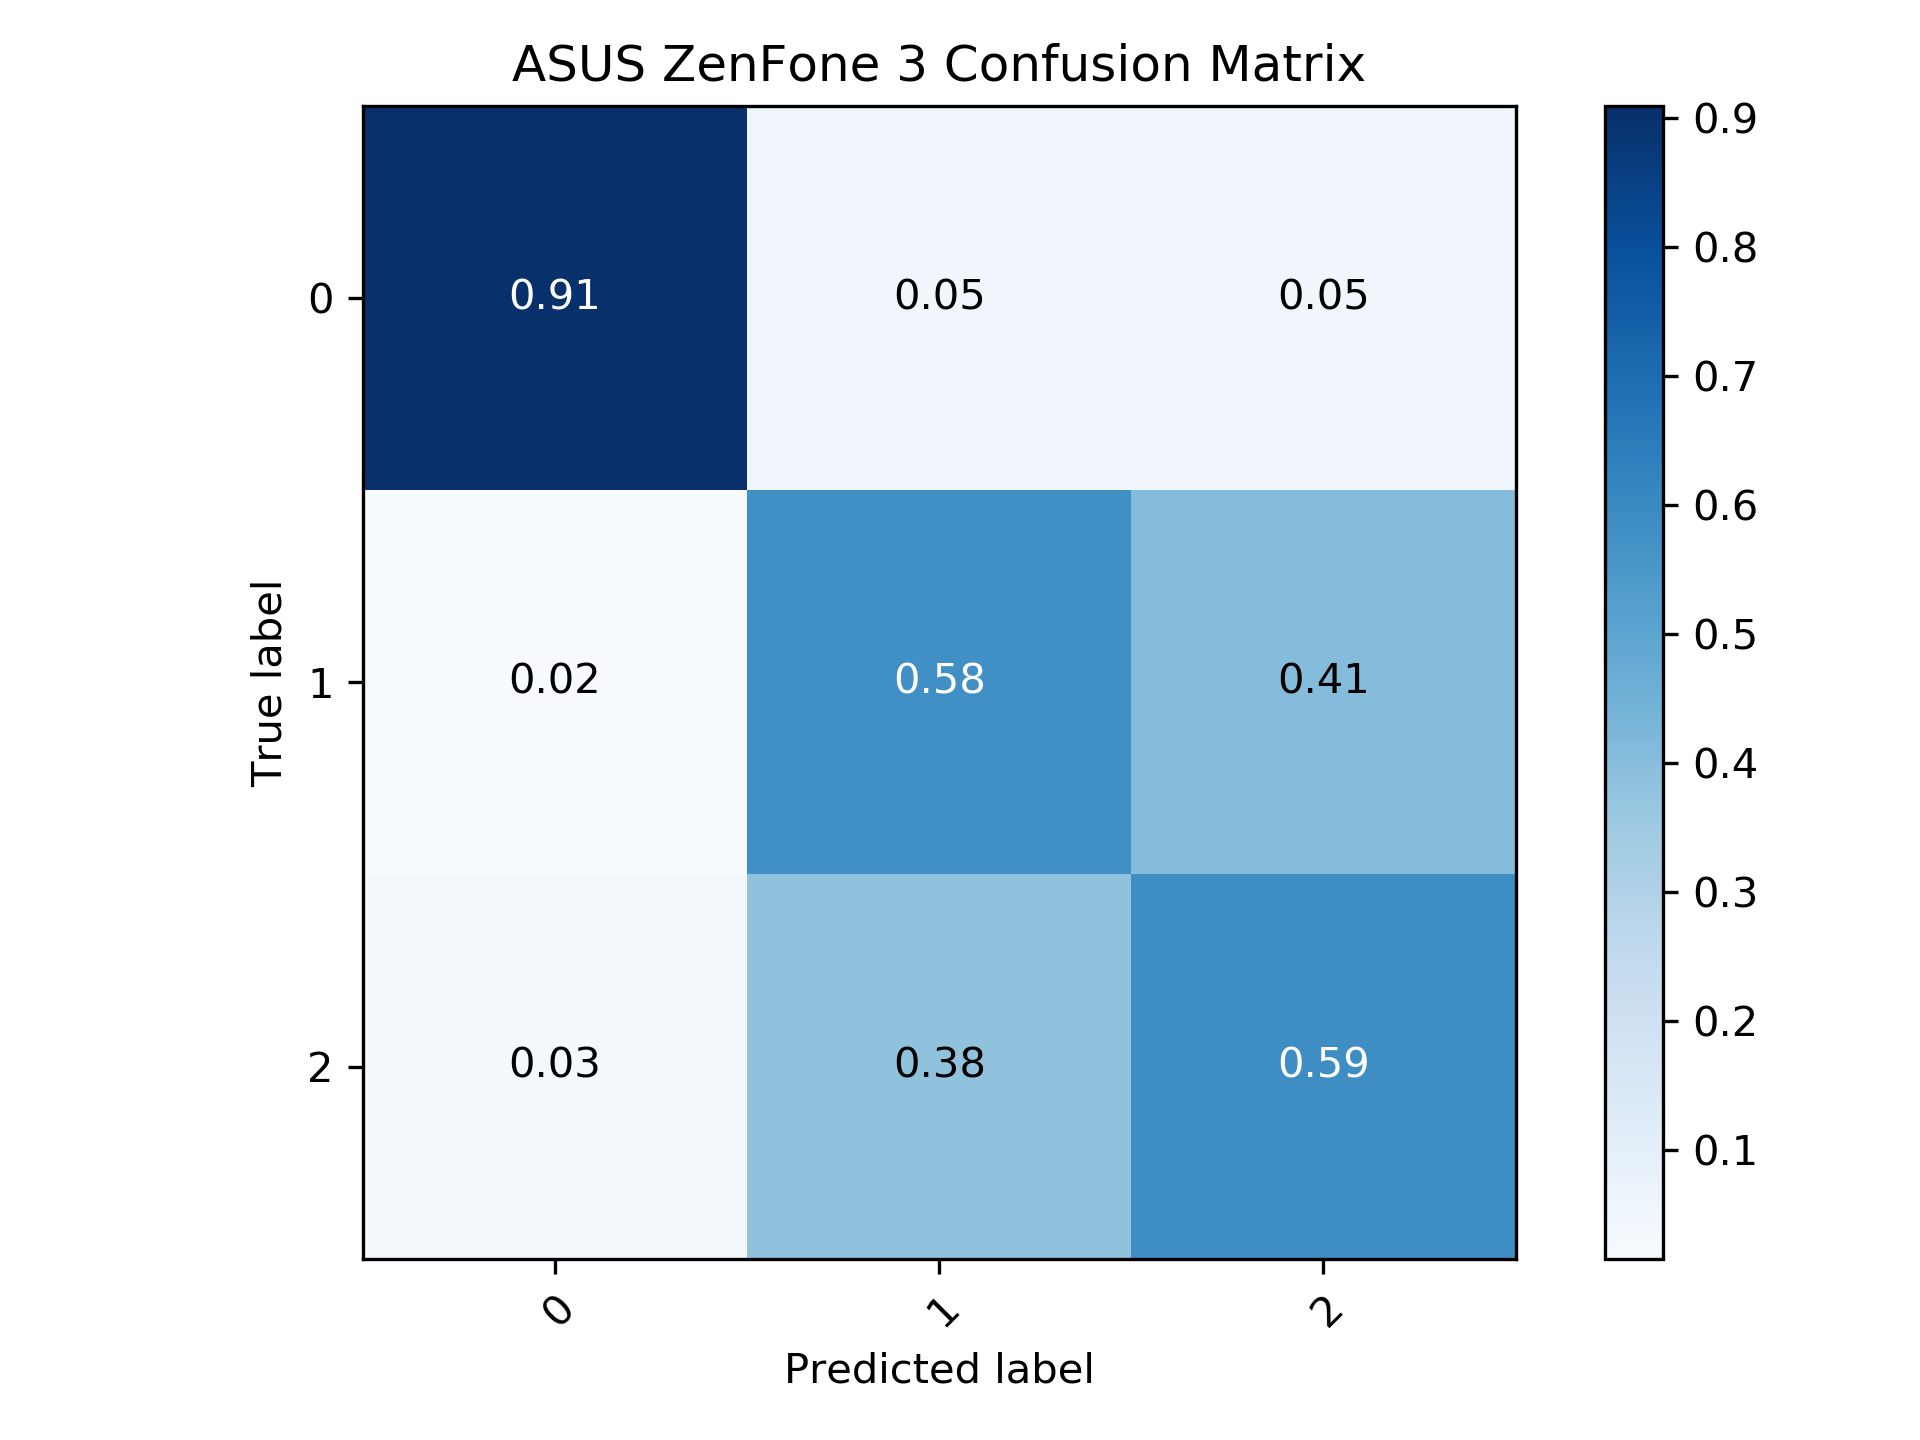
\includegraphics[width=0.67\linewidth]{ExperimentalResults/scaled_cm.png}}
\caption{Confusion Matrix for Recompression Classification using Scaled Data}
\label{scaledcm}
\end{figure}